% vim: set textwidth=78 autoindent:

\subsection{Schnelldruck Plugin}

% when the revision of a section has been finalized, 
% comment out the following line:
% \updatedisclaimer

Das Plugin \toolbtntwo{quick_print}{Schnelldruck} Plugin erlaubt es, das
aktuelle Kartenfenster mit minimalem Aufwand in ein PDF zu exportieren. Der
Benutzer gibt dazu nur einen Kartentitel, einen Kartennamen und die
Seitengr��e an (siehe Abbildung~\ref{fig:quickprint})

\begin{figure}[ht]
   \begin{center}
   \caption{Schnelldruck Dialog \nixcaption}\label{fig:quickprint}\smallskip
   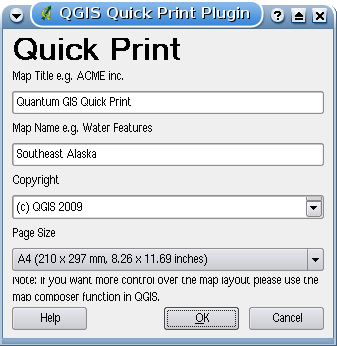
\includegraphics[clip=true, width=6cm]{quick_print_dialog}
\end{center}
\end{figure}

Abbildung~\ref{fig:quickprint_result} zeigt einen DIN A4 Schnelldruck mit
Layern des QGIS Beispieldatensatzes. F�r mehr Kontrolle �ber das Kartenlayout
steht das Print Composer Plugin (siehe Kapitel~\ref{label_printcomposer}) zur Verf�gung.

\begin{figure}[ht]
   \begin{center}
   \caption{DIN A4 Schnelldruck als PDF\nixcaption}\label{fig:quickprint_result}\smallskip
   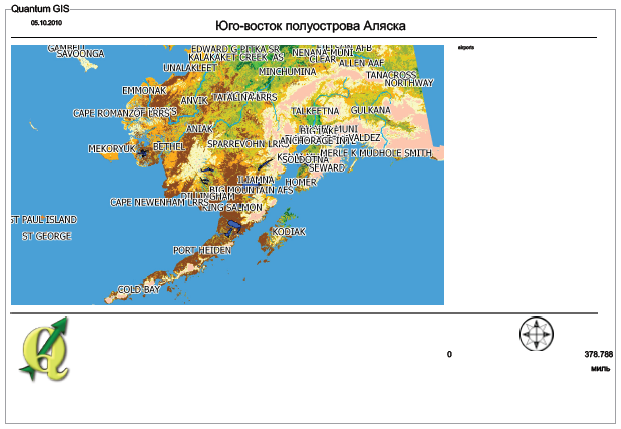
\includegraphics[clip=true, width=9cm]{quick_print_result}
\end{center}
\end{figure}


